%\section{Summary of the Work}
%{\LARGE T}







\section{Introduction}\label{}

In our previous work  rPPG has been Investigate for stress estimation through some physiological parameter were we found that 
 for the stress estimation there are variability exist in rPPG signal, In recent studies have begun to investigate its potential as a biometric identifier. For example, Sun et al.~\cite{sun2024biometric} demonstrated that de-identified rPPG signals, independent of facial features can be used for biometric identification.In Biometric systems require the permanence of the signal under all conditions, while stress detection depends on signal variability~\cite{sun2024biometric}\cite{icpram25} as depicted in Figure~\ref{fig:contradict}. This contradictory requirement challenges the feasibility of rPPG as a reliable biometric modality. Specifically, in this paper, we aim to answer the following two questions: (1) Can we use rPPG signals as a biometric identity or not . (2) If yes, then under what physiological state. Our findings  broadly contribute to the broader understanding of whether rPPG can serve as a viable biometric modality despite its dynamic physiological nature.
\begin{figure}[!htp]  % [h!] places the figure approximately here
    \centering
    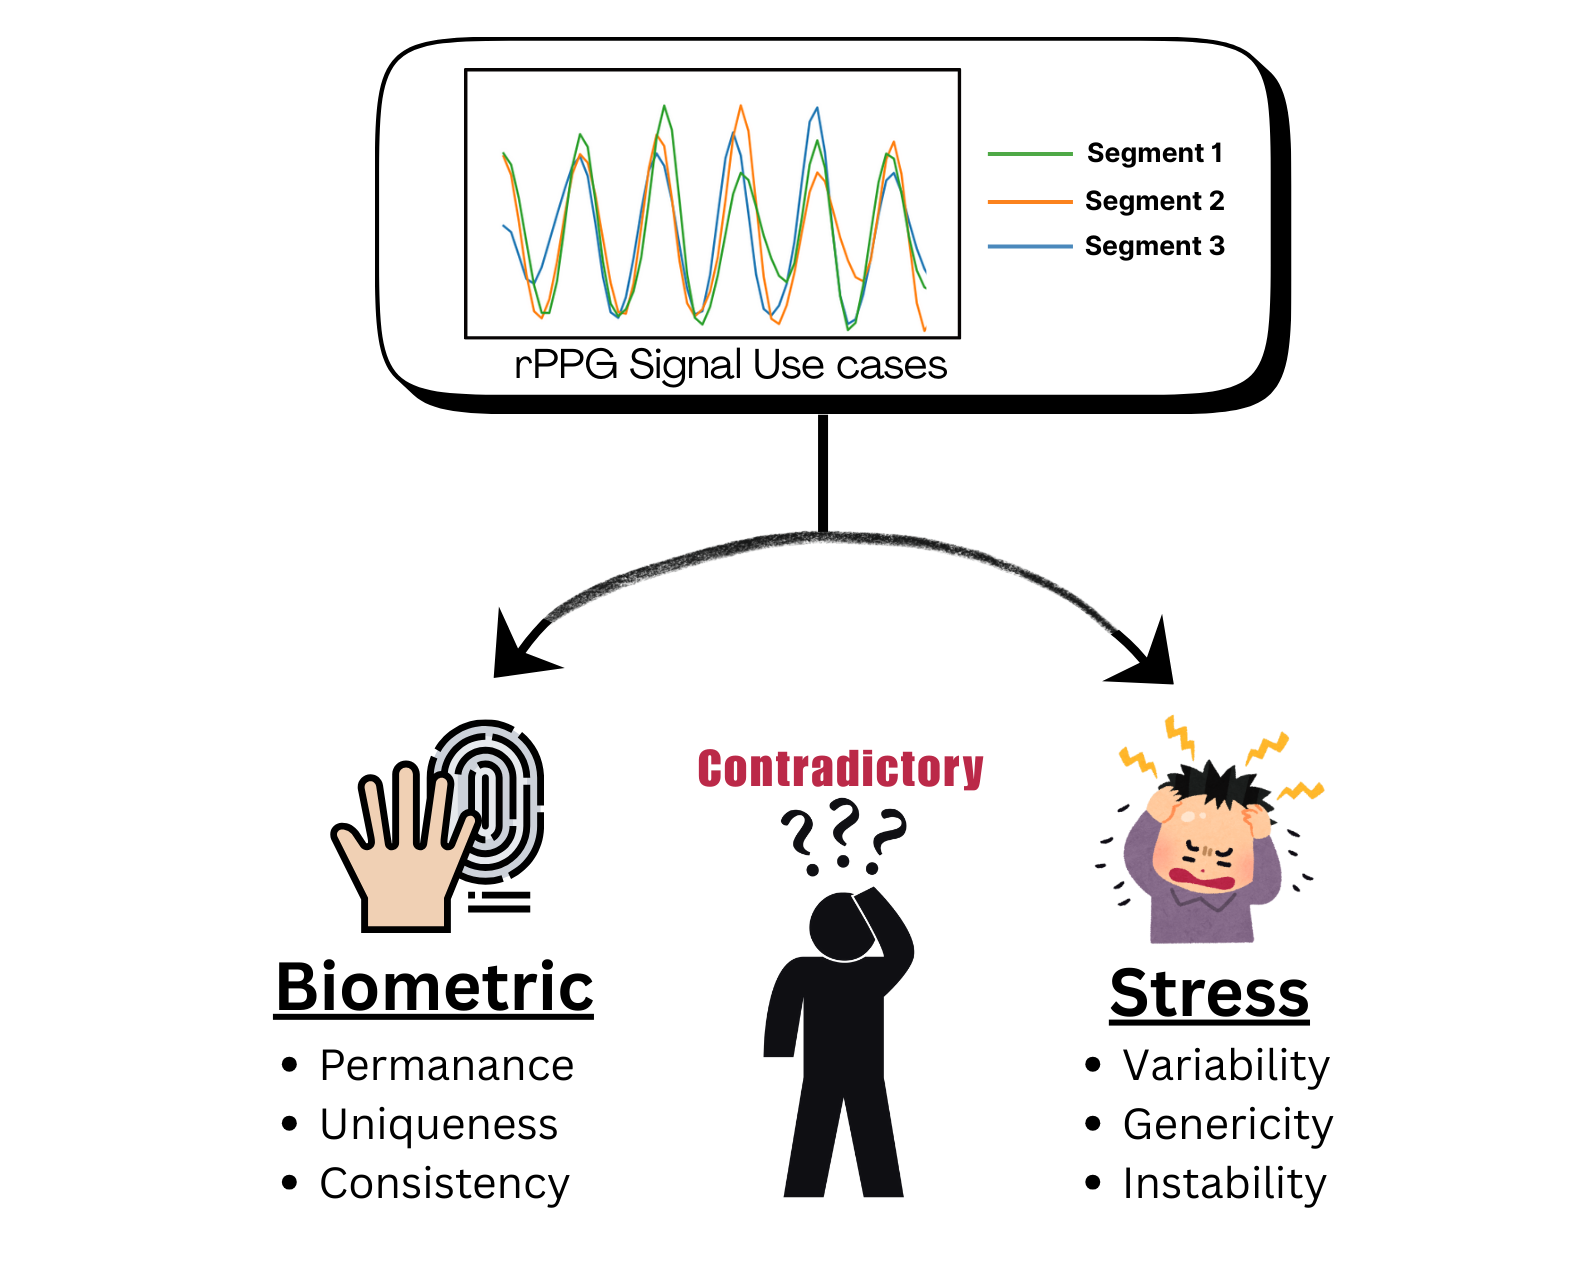
\includegraphics[width=0.8\textwidth, height=0.4\textheight]{Chapter2/Figures/Biometric (2).png}  % Adjust the width as needed
    \caption{Illustration of the uncertainty in using rPPG signals for biometric identification.}
    \label{fig:contradict}  % Label for referencing the image
\end{figure}


The key contributions of this work are summarized as follows:

\begin{itemize}
    \item \textbf{Identity Consistency Under Physiological Variability:} We investigate whether an individual’s rPPG-based biometric identity remains stable across varying physiological states, such as normal and stress-induced conditions. Through extensive testing, we demonstrate that physiological changes significantly impact the consistency of rPPG features used for identification.
    \item \textbf{Identity Robustness Under Motion Condition:}We studied the resilience of biometric systems based on rPPG against practical distortions such as head motion and lighting variations. This study provides important information on the limitations of the rPPG biometrics under stress and motion.

   % \item \textbf{Robustness to Real-world Distortions Through Cross-Dataset Evaluation:} We study the resilience of rPPG-based biometric systems against practical distortions such as head motion and lighting variations, and validate our approach across three diverse public datasets (PURE, UBFC-Phys, and MSPM). This evaluation highlights the challenges of maintaining identification accuracy in uncontrolled, real-world conditions and provides important insights into the limitations of rPPG biometrics under stress and motion.
   \item \textbf{Rigorous Experimentation:} We have conducted rigorous experimentation with three diverse publicly available datasets (PURE, UBFC-Phys and MSPM) to determine the effectiveness of the proposed technique.

   % \item \textbf{CNN-Based Embedding Model with Triplet Loss for Biometric Discrimination:} We propose a CNN-based framework trained with a hard triplet loss function to extract discriminative heartbeat-level rPPG embeddings. Our model effectively learns identity-specific representations, even when trained on short and noisy physiological signal segments.
\end{itemize}




The remainder of this paper is organized as follows: Section 2 gives a brief introduction to biometrics (nontraditional modalities). Section 3 outlines the proposed methodology for rPPG-based biometric identification. Section 4 details the experimental setup and datasets. Section 5 discusses the results and performance analysis. Finally, Section 6 concludes the study and outlines directions for future research.






    
\section{Related Work}
 Traditionally, biometric identification systems have relied on physiological characteristics such as fingerprints, iris patterns, and facial features to identify an individual~\cite{shaheed2021systematic}.  These modalities have been thoroughly examined in a number of studies.  For example, \cite{taigman2014deepface} presented a face verification system that integrates 3D frontalization techniques for increased accuracy and uses a deep neural network trained on 4,000 IDs. In~\cite{nguyen2024deep}, the author emphasized the distinct and stable texture of the iris for iris recognition. This texture is created before birth and has a high degree of genotypic variability, making it a highly reliable biometric authentication method.  In order to improve accuracy and scalability in practical  applications, \cite{arslan2025analytical} suggested an analytical system architecture for  fingerprint examination that incorporates cutting-edge feature extraction and pattern matching techniques. 
 
 In the current era, biometric researchers are now focusing on exploring the potential of nontraditional modalities like photoplethysmography (PPG), electrocardiography (ECG), and remote photoplethysmography (rPPG) as biometric identifier. Like in~\cite{cherry2024optimizing} author's integrate PPG signals in biometric systems for liveness detection. In their work~\cite{cherry2024optimizing} they have used both the 1D and 2D representation of PPG signals for biometric identification. In~\cite{kim2025utilization} authors utilize electrocardiogram (ECG) signals for biometric authentication by leveraging their unique physiological properties for user identification. They propose a two-stage ECG-based biometric identification system. In the first stage, ECG signals are preprocessed to extract features such as amplitude, shape, and waveform. The signals are then classified into two categories: stable (normal) and unstable (stressed). In the second stage, the model combines the raw ECG signal with the output from the first stage to improve identification accuracy. However, the system still has some limitations. For instance, if the first-stage model misclassifies the user's state, it may negatively impact identification performance. Moreover, the model has limited representation of real-world variability, such as cognitive stress, disease conditions, and age-related changes. Very recently, Sun et al. ~\cite{sun2024biometric},  presented an rPPG-based approach for biometric authentication  which focuses on rPPG signal extraction from de-identified facial videos. In their work, they have  utilized  both rPPG morphological information and external contact photoplethysmography(cPPG)-based biometric data. They proposed  a two-stage training strategy to improve rPPG signal morphology and accomplish precise biometric authentication. However, its applicability as a biometric identifier under physiological variability and robustness under motion condition is still questionable. In, this work we aim to answer aforementioned raised question.






\section{METHODOLOGY}

This section discusses the proposed framework, which consists of three main modules: (i) Region of Interest (ROI) segmentation, (ii) rPPG signal extraction, and (iii) the proposed feature extractor. These modules are described in detail in the following sections.

For Modules (i) and (ii), we adopt a similar approach to the one used in our previous study titled \textit{Non-contact Stress Estimation Using Deep Tabular Methods}. The network architecture used is illustrated in Figure~\ref{fig:CNN architecture1}. Once the rPPG signal is extracted by following the method from our earlier study then apply signal quantization techniques, also depicted in Figure~\ref{fig:CNN architecture1}, as part of Module (ii).

In the signal quantization step, the rPPG signal is segmented into overlapping windows based on a fixed number of heartbeats—specifically, 5, 10, and 20 beats as described in~\cite{sun2024biometric}. These segments are defined using systolic peaks identified from the filtered rPPG signal. Due to individual variations in heart rate, the duration of each segment and consequently, the number of samples per segment varies depending on the interval between the first and last detected beats.

To address this inconsistency and enable uniform analysis across subjects and segment lengths, each segment is linearly interpolated to a fixed length of 90 samples. Formally, for a given signal segment $s = \{s_1, s_2, \ldots, s_n\}$ of arbitrary length $n$, we compute a continuous interpolation function $f(x)$ over the normalized interval $x \in [0, 1]$, and then resample it at 90 evenly spaced points:
\[
x_\text{target} = \left\{ \frac{i}{89} \mid i = 0, 1, \ldots, 89 \right\}, \quad s' = f(x_\text{target})
\]
This choice of 90 samples ensures that the interpolated segment accommodates even the slowest plausible heart rate (down to 40 BPM), thereby maintaining signal periodicity and comparability across all segments.

\begin{figure*}[!htp]
    \centering
    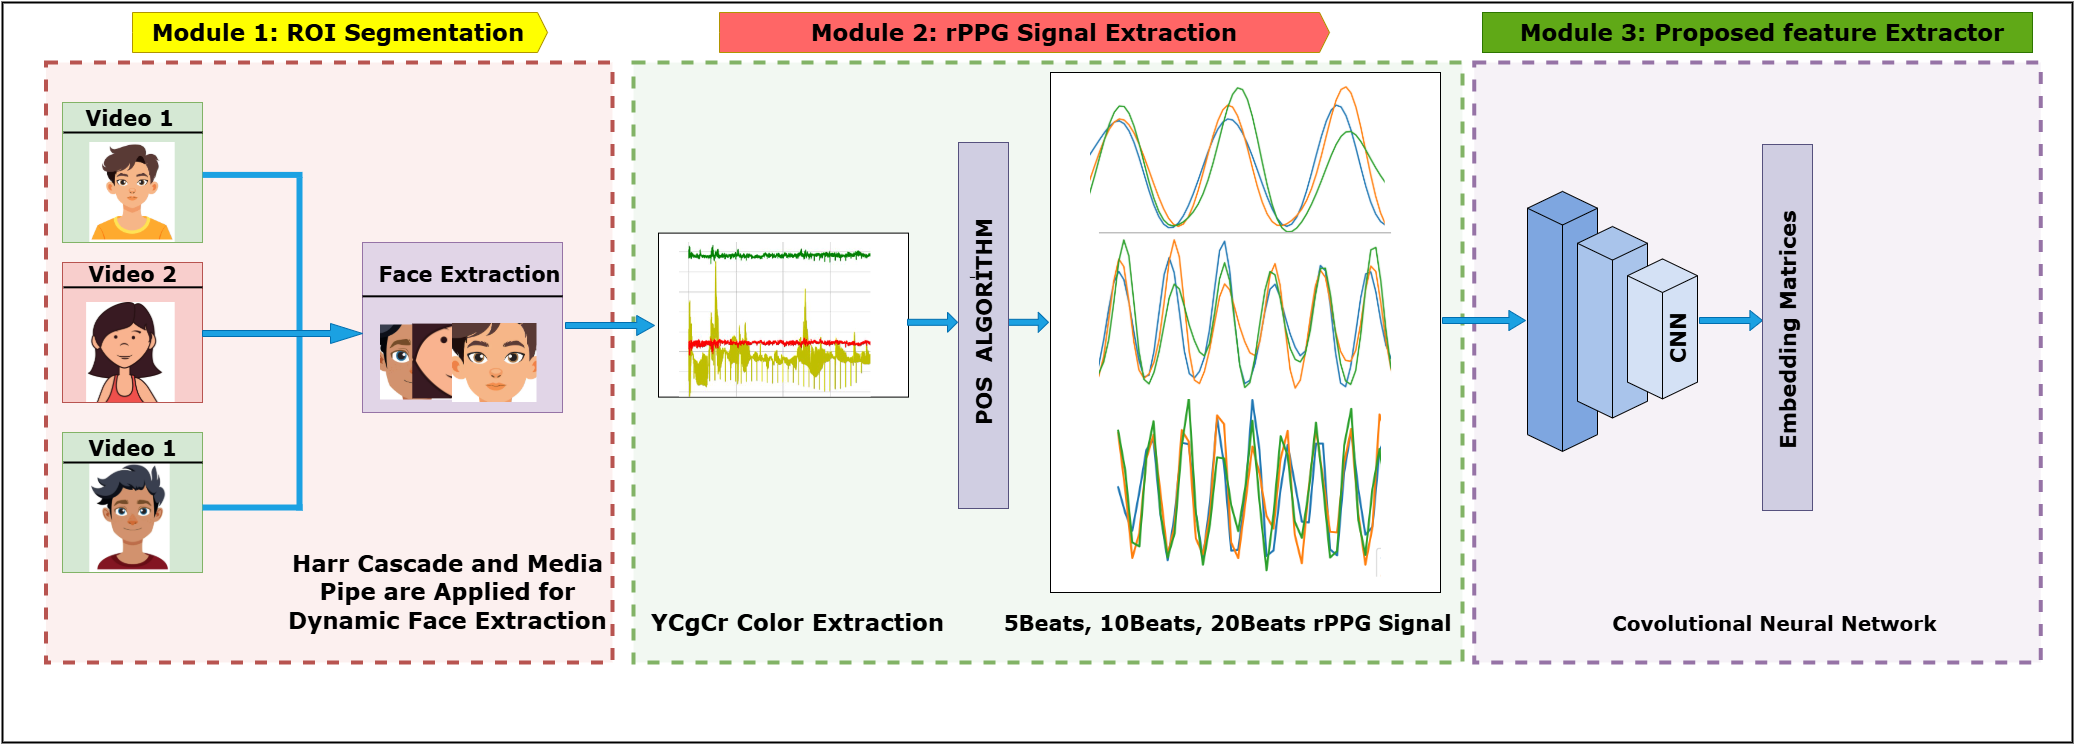
\includegraphics[width=\textwidth]{Chapter2/Figures/Cnn_embedding_model.png}
    \caption{CNN-Based Embedding model}
    \label{fig:CNN architecture1}
\end{figure*}








\subsection{Proposed Feature Extractor}
Once the rPPG signals are extracted next step is to learn robust and discriminative features from it. To achieve this, we have employed a convolutional neural network (CNN) based embedding model trained using metric learning paradigm. The network architecture is depicted in Figure~\ref{fig:CNN architecture}. This network takes 1D segment of fixed length($90$ samples) as input and passed it to three convolutional blocks. Table 1 illustrates complete architectural details of proposed feature extractor. The output of last convolutional layer is flattened to generate $128$ dimensional feature vector. Instead of training our proposed feature extractor as a classifier we have trained it as a metric using triplet loss with hard negative mining as depicted in equation~\ref{eq:triplet_loss}.
\begin{equation}
\mathcal{L}_{\text{triplet}} = \max \left( \|f(x^{rPPG_a}) - f(x^{rPPG_p})\|_2^2 - \min_j \|f(x^{rPPG_a}) - f(x^{rPPG_n}_j)\|_2^2 + \alpha, 0 \right)
\label{eq:triplet_loss}
\end{equation}

Here, \( x^{rPPG_a} \), \( x^{rPPG_P} \), and \( x^{rPPG_n}_j \) represent the anchor, positive, and hard negative rPPG signals  respectively, and \( \alpha \) is the margin hyperparameter. This formulation encourages the network to learn embeddings such that signals from the same subject are closer in the embedding space, while signals from different subjects are farther apart.

\textbf{Network Parameter Optimization} the hyperparameters of the proposed network are calculated empirically over a small validation set and they are as: initial learning rate = $0.001$, optimizer =Adam, margin=$1.0$ , batch size= $10$.

\begin{table}[h!]
\centering
\caption{CNN Architecture Details of the Proposed Feature Extractor}
\begin{tabular}{|l|c|c|c|}
\hline
\textbf{Layer} & \textbf{Kernel Size} & \textbf{Stride} & \textbf{Output Channels} \\
\hline
Conv1          & 5 $\times$ 5         & 1               & 32                        \\
BatchNorm1     & -                   & -               & 32                        \\
LeakyReLU1     & -                   & -               & 32                        \\
MaxPooling1    & 2 $\times$ 2        & 2               & 32                        \\
\hline
Conv2          & 3 $\times$ 3         & 1               & 64                        \\
BatchNorm2     & -                   & -               & 64                        \\
LeakyReLU2     & -                   & -               & 64                        \\
MaxPooling2    & 2 $\times$ 2         & 2               & 64                        \\
\hline
Conv3          & 3 $\times$ 3         & 1               & 128                       \\
BatchNorm3     & -                   & -               & 128                       \\
LeakyReLU3     & -                   & -               & 128                       \\
MaxPooling3    & 2 $\times$ 2         & 2               & 128                       \\
\hline
Flatten        & -                   & -               & $(\text{input\_size} / 8) \times 128$ \\
Linear1 (FC1)  & -                   & -               & 512                        \\
BatchNorm4     & -                   & -               & 512                        \\
LeakyReLU4     & -                   & -               & 512                        \\
Dropout        & -                   & -               & -                          \\
Linear2 (FC2)  & -                   & -               & 128                        \\
L2 Normalize   & -                   & -               & 128                        \\
\hline
\end{tabular}
\label{tab:cnn_architecture1}
\end{table}
For the validation phase, we employ a distance-based evaluation protocol to measure how closely the embedding of a test segment matches those of the known training subjects. Specifically, we use Euclidean distance by considering the equation\ref{eq:ecl_dis} as a similarity metric to compare each test embedding against the pre-computed subject-wise mean embeddings obtained during training. Let $\mathbf{z}_t$ denote the embedding of a test segment and $\{\mathbf{z}_s^{(i)}\}_{i=1}^N$ be the set of reference embeddings from $N$ enrolled subjects. The similarity between the test embedding and a reference subject $i$ is computed using the negative Euclidean distance:

\begin{equation}
\text{score}^{(i)} = -\|\mathbf{z}_t - \mathbf{z}_s^{(i)}\|_2
\label{eq:ecl_dis}
\end{equation}


This negative formulation allows the distances to be used directly for similarity ranking, where higher scores indicate greater similarity.

\section{Experimental Details }  This section provides details about the database used along with its training and testing protocol. Moreover, this section also provides details about the set-up process of our simulation environment.

\subsection{Dataset Description} 
We conduct our experiments on three datasets, namely PURE~\cite{ferrari2017pure}, Ubfc-Phy~\cite{sabour2023ubfc}, and  MSMP~\cite{speth2024mspm}. The PURE dataset~\cite{ferrari2017pure} comprises recordings of 10 subjects (8 male, 2 female) performing controlled head movements under six different motion setups, including steady gaze, talking, translation (slow/fast), and head rotations (small/medium). Each subject was recorded in three lighting conditions, resulting in 60 one-minute video sequences. Videos were captured at 30 Hz with a resolution of 640×480 pixels, while reference pulse data was recorded at 60 Hz using a finger clip pulse oximeter. The setup simulates a natural head movements under varying illumination.

The UBFC-Phys dataset~\cite{sabour2023ubfc} is a multimodal dataset created for psychophysiological research under social stress. It features data from 56 participants who each completed three tasks—rest (T1), speech (T2), and arithmetic (T3)—while being recorded on video and monitored for physiological responses. Each video is 3 minutes long and was recorded at 30 Hz using an EO-23121C camera. Participants were randomly assigned to either a control or test condition, and self-reported anxiety and confidence scores were collected before and after the experiment. The dataset includes subject information, video recordings for each task, and self-assessment scores.

The Multi-Site Physiological Monitoring (MSPM) dataset~\cite{speth2024mspm} captures multimodal physiological data from subjects performing various tasks, including controlled activities like breath-holding and adversarial visual stimuli for rPPG testing. Each session includes synchronized recordings from multiple sources: RGB videos from three camera angles (front, top, and iPhone), near-infrared (NIR) videos. 
In our study we have employed the same training and testing protocol as used by latest state-of-the art work~\cite{sun2024biometric}. The intra-session test uses data recorded within the same session, while the cross-session test uses data from different sessions. 

For the PURE dataset, we have  divided the steady session into two parts: the first 60\% of the sequence is used for training, and the remaining 40\% is used for intra session testing. The head motion data are used for cross-session testing. 

In the UBFC-rPPG dataset, the same division(60\% training and 40\% Testing) is applied to each video of rest task (T1) which is used for intra-session testing, and the arithmetic task (T3) is used for cross-session testing. 

For the MSPM dataset, RGB front-view recordings are used for intra session testing, while RGB top-view recordings are used for cross-session testing, with the same 60/40 division applied. 


\subsection{Experimental Setup }
Our CNN model is trained on a system with the following configuration: Intel(R) Xeon(R) Silver 4114 CPU, 64 GB RAM, 4 TB SSD, and two NVIDIA GeForce GTX 1080 Ti GPUs.  During inference, predicted probabilities from consecutive periodic segments (5 beats, 10 beats, and 20 beats) are averaged to produce the final output.


\section{Results and Discussion}
\subsection{Performance Evaluation}

A one-vs-rest strategy is employed for performance evaluation. In this approach, each subject is treated as the positive class (genuine), while all other subjects are considered as the negative class (impostors). For every subject, we collect similarity scores from all validation samples and assign binary labels based on whether a sample belongs to the target subject (genuine) or to another subject (impostor).

\begin{figure}[h!]
    \centering
    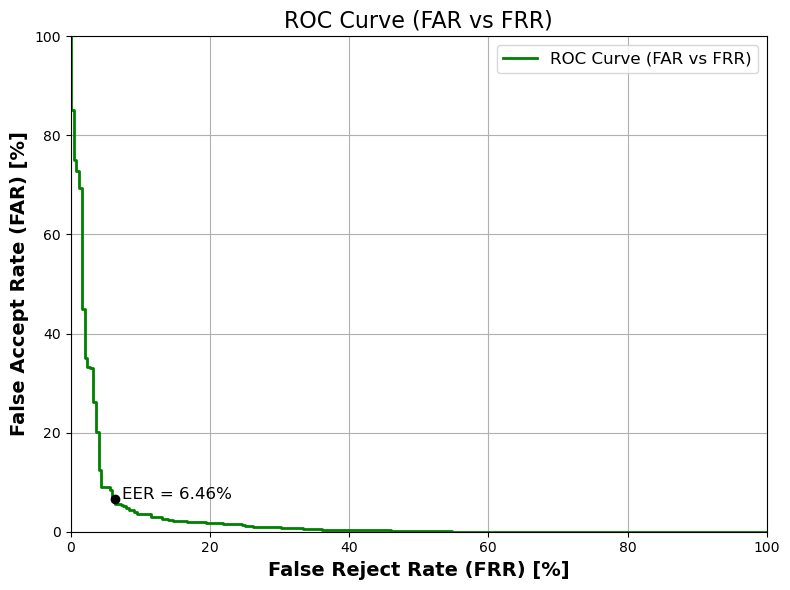
\includegraphics[width=0.7\textwidth]{Chapter4/Figures/ROC_pure20.png}
    \caption{Graphical representation of the Equal Error Rate (EER) calculated for the 5-bit Pure Dataset.}
    \label{fig:roc_5bit_pure}
\end{figure}

To evaluate model performance, we use standard metrics such as the Equal Error Rate (EER) and the Area Under the Receiver Operating Characteristic Curve (AUC). A lower EER and a higher AUC reflect better classification performance, indicating the model's ability to effectively distinguish between genuine and impostor samples. The ROC Curve on the PURE dataset are presented in Figure~\ref{fig:roc_5bit_pure}.
%Additionally, the number of genuine and impostor records is summarized in Table~\ref{tab:Gen_emposter}. These results are derived from the 5-bit quantization segment across all three datasets: PURE, UBFC-Phys, and MSPM. During validation intra-session, multiple segments may exist for each subject. If at least 30\% of the  validation segments match the mean embedding of the corresponding subject, the sample is treated as a genuine match.




% \begin{table}[h]
% \centering
% \caption{Genuine and Imposter records for 5-bit quantization on three datasets}
% \begin{tabular}{|c|c|c|c|}
% \hline
% \textbf{Dataset} & \textbf{Classes} & \textbf{Genuine} & \textbf{Imposter}  \\ \hline
% Pure & 10 & 9 & 1 \\ \hline
% UBFc-Phy & 56 & 11 & 45 \\ \hline
% MSMP & 15 & 1 & 14 \\ \hline
% \end{tabular}
% \label{tab:Gen_emposter}
% \end{table}



\subsection{Impact of Quantization on rPPG Signal Representation}

This section presents a visual comparison of rPPG signals extracted from the PURE dataset using three different quantization levels: 5-bit, 10-bit, and 20-bit. For each bit level, we examine the signals under two conditions: stable (minimal motion) and head motion.
\begin{figure}[h!]
    \centering

    \subfigure[rPPG signal under stable condition (5-bit quantization).]{
        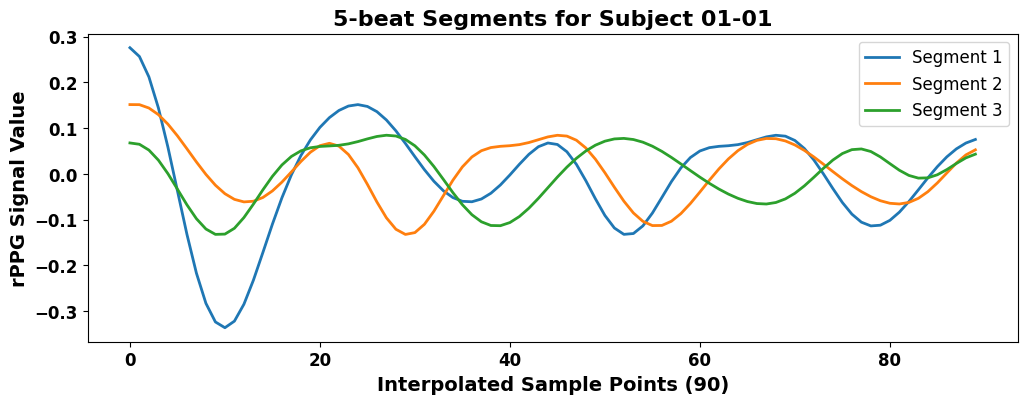
\includegraphics[width=0.48\textwidth]{Chapter2/Figures/5_bit_Stable_pure.png}
        \label{fig:rppg_stable}
    }
    \hfill
    \subfigure[rPPG signal under head motion condition (5-bit quantization).]{
        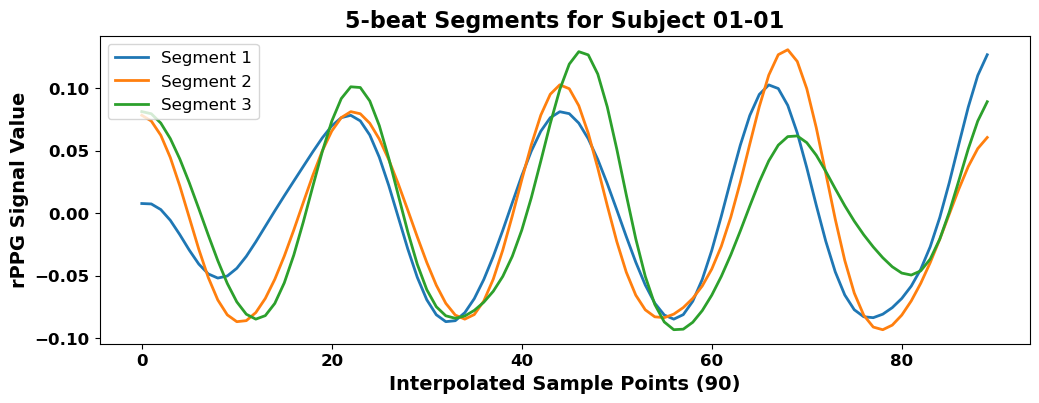
\includegraphics[width=0.48\textwidth]{Chapter2/Figures/5_bit_HM_pure.png}
        \label{fig:rppg_hm}
    }

    \caption{Comparison of extracted rPPG signals for stable and head motion conditions on the PURE dataset using 5-bit quantization.}
    \label{fig:rppg_comparison_conditions}
\end{figure}
\begin{figure}[h!]
    \centering

    \subfigure[rPPG signal under stable condition (10-bit quantization).]{
        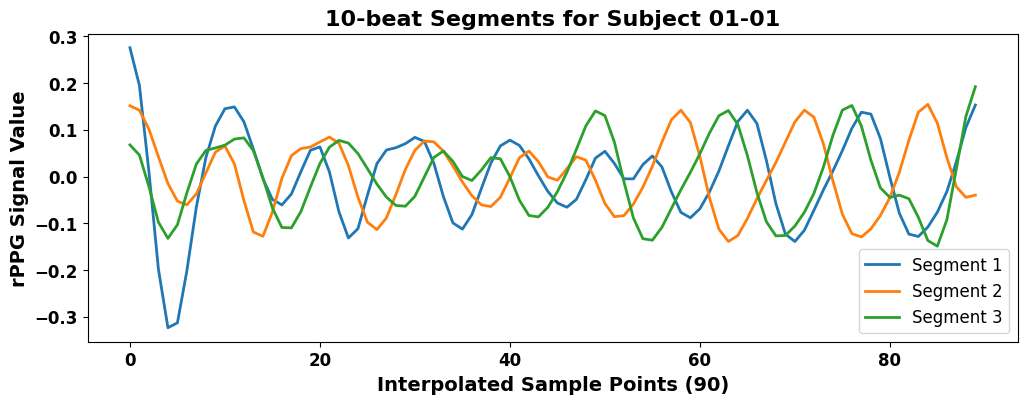
\includegraphics[width=0.48\textwidth]{Chapter2/Figures/10_bit_stable _pure.png}
        \label{fig:rppg_stable}
    }
    \hfill
    \subfigure[rPPG signal under head motion condition (10-bit quantization).]{
        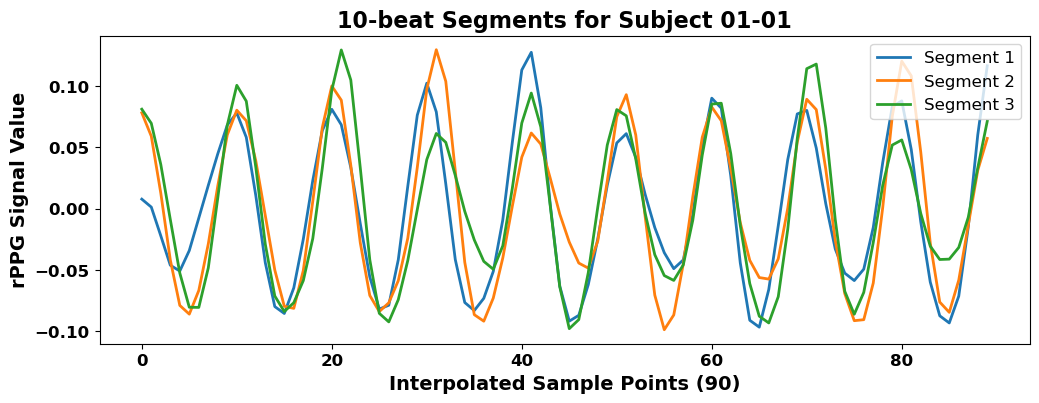
\includegraphics[width=0.48\textwidth]{Chapter2/Figures/10_bit_HM_Pure.png}
        \label{fig:rppg_hm}
    }

    \caption{Comparison of extracted rPPG signals for stable and head motion conditions on the PURE dataset using 10-bit quantization.}
    \label{fig:rppg_comparison_conditions1}
\end{figure}
\begin{figure}[h!]
    \centering

    \subfigure[rPPG signal under stable condition (20-bit quantization).]{
        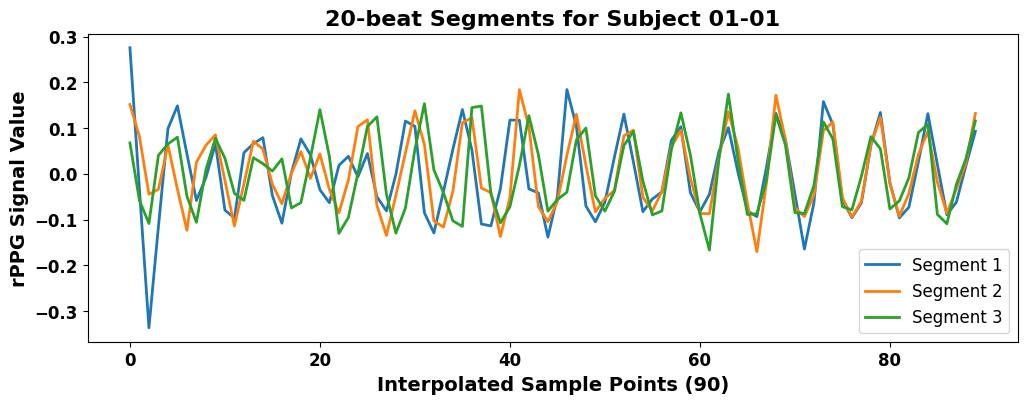
\includegraphics[width=0.48\textwidth]{Chapter2/Figures/20_bit_stable_pure.png}
        \label{fig:rppg_stable}
    }
    \hfill
    \subfigure[rPPG signal under head motion condition (20-bit quantization).]{
        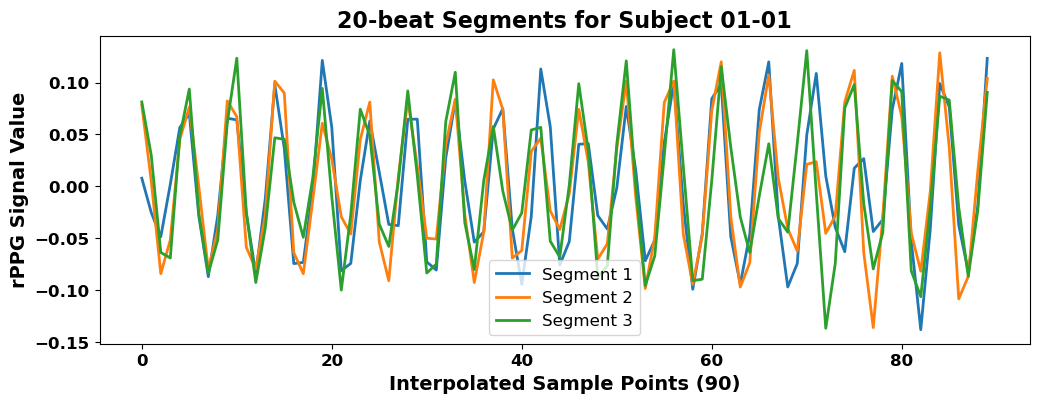
\includegraphics[width=0.48\textwidth]{Chapter2/Figures/20_bit_HM_Pure.png}
        \label{fig:rppg_hm}
    }

    \caption{Comparison of extracted rPPG signals for stable and head motion conditions on the PURE dataset using 20-bit quantization.}
    \label{fig:rppg_comparison_conditions2}
\end{figure}

Figure~\ref{fig:rppg_comparison_conditions} displays the 5-bit rPPG signals, where subfigures (a) and (b) correspond to the stable and head motion conditions, respectively. Figure~\ref{fig:rppg_comparison_conditions1} and Figure~\ref{fig:rppg_comparison_conditions2} present similar comparisons for the 10-bit and 20-bit quantized signals.

Across all bit depths, the signals under stable conditions appear smoother and more consistent in waveform, while the head motion scenarios show increased variability and mild distortion—particularly at lower bit depths. However, even the 5-bit quantized signals preserve key periodic features of the pulse waveform, demonstrating the effectiveness of the proposed pipeline under aggressive compression.

Notably, the visual integrity of the rPPG signal is well-maintained across all quantization levels, especially under stable conditions. This suggests that lower-bit quantization may be a viable trade-off for resource-constrained biometric systems, without severely degrading signal quality.

\subsection{t-SNE Visualization of Learned Embeddings}
To qualitatively evaluate the discriminative power of the learned embeddings, we perform a 2D t-SNE (t-distributed stochastic neighbor embedding) visualization for each quantization level: 5-bit, 10-bit, and 20-bit of PURE data. These visualizations help illustrate how well the proposed CNN model clusters feature representations of different subjects in the reduced embedding space.
\begin{figure}[h!]
    \centering
    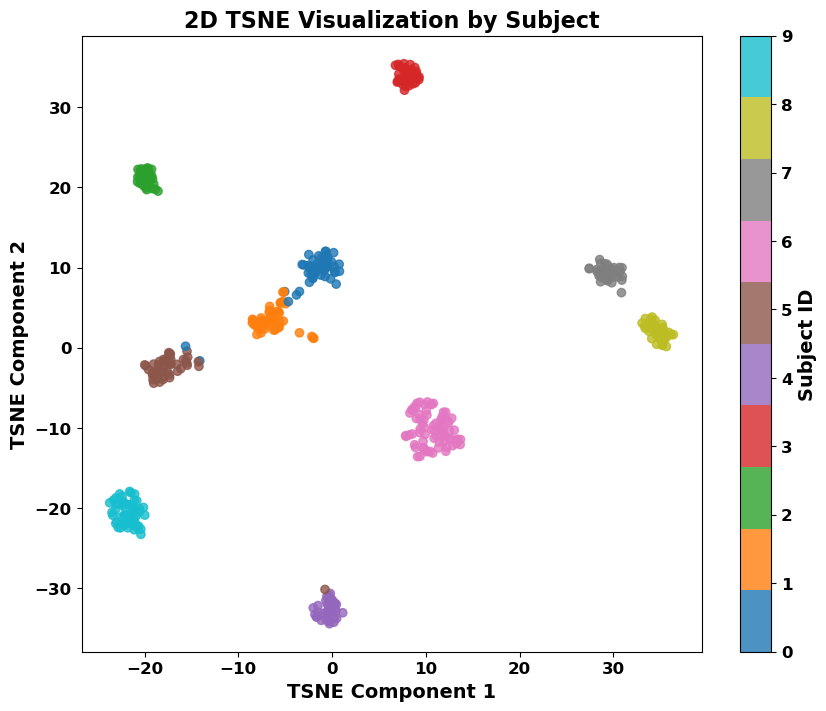
\includegraphics[width=0.7\textwidth, height=0.5\textwidth]{Chapter2/Figures/tsne_5bit_pure_stable.png}
    \caption{t-SNE visualization of 5-bit quantized embeddings on the PURE dataset (stable condition).}
    \label{fig:tsne_5bit_pure}
\end{figure}

As shown in Figures~\ref{fig:tsne_5bit_pure}, \ref{fig:tsne_10bit_pure}, and \ref{fig:tsne_20bit_pure}, the embeddings from all three quantization levels exhibit distinct clustering patterns, indicating the model’s ability to capture subject-specific features effectively, even at lower bit depths. The 20-bit representation shows well-separated and compact clusters, suggesting high discriminability. Interestingly, even the 5-bit embedding space shows meaningful clustering, with minimal overlap between classes—highlighting the robustness of the proposed method under quantization constraints.

These results confirm that the learned feature space preserves identity information across different quantization levels, demonstrating the feasibility of lightweight biometric systems with low-bit precision while maintaining strong separability among subjects.



\begin{figure}[h!]
    \centering
    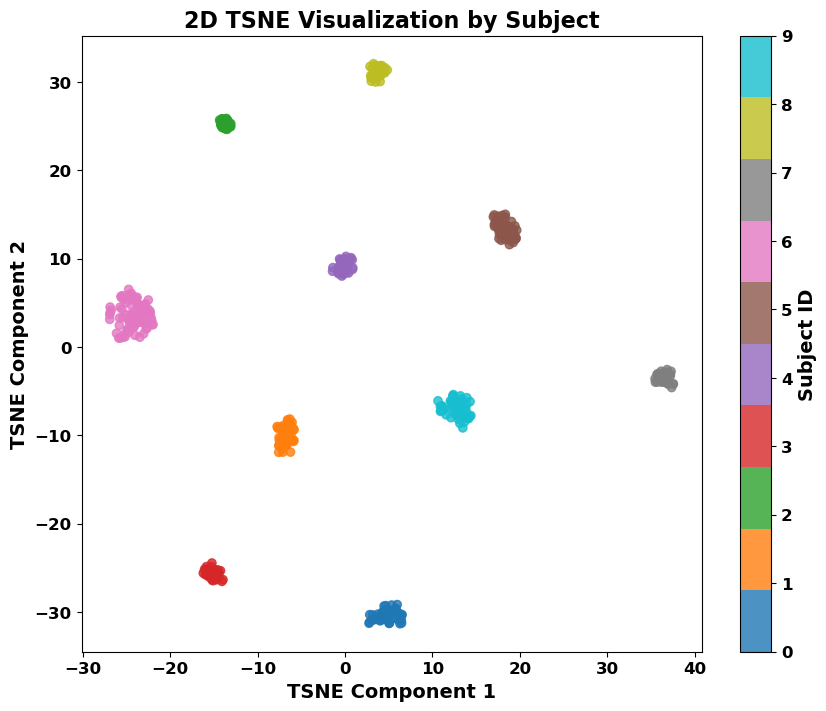
\includegraphics[width=0.7\textwidth, height=0.5\textwidth]{Chapter2/Figures/tsne_10bit_pure_stable.png}
    \caption{t-SNE visualization of 10-bit quantized embeddings on the PURE dataset (stable condition).}
    \label{fig:tsne_10bit_pure}
\end{figure}

\begin{figure}[h!]
    \centering
    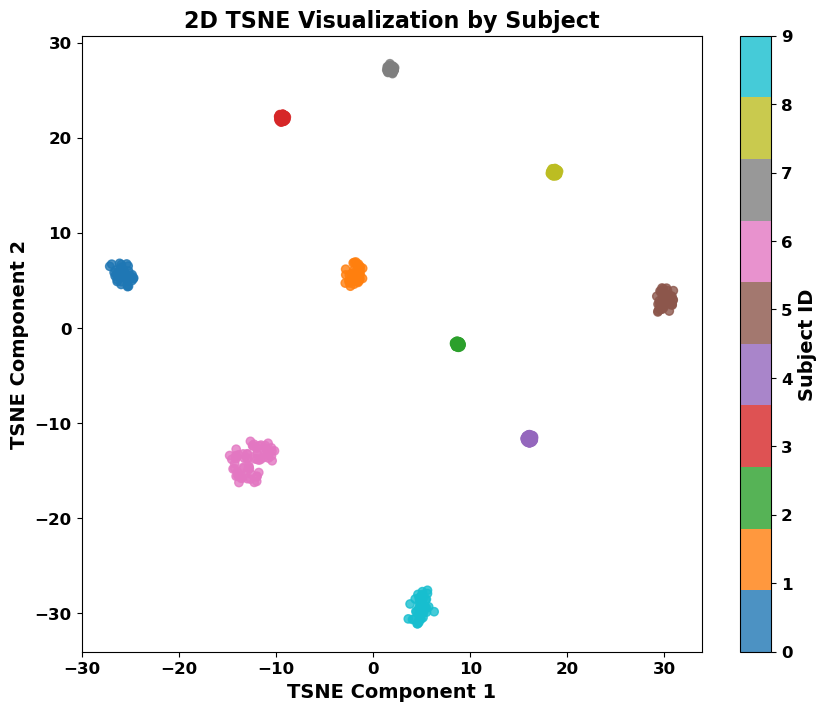
\includegraphics[width=0.7\textwidth,  height=0.5\textwidth]{Chapter2/Figures/tsne_20_bit_pure_stable.png}
    \caption{t-SNE visualization of 20-bit quantized embeddings on the PURE dataset (stable condition).}
    \label{fig:tsne_20bit_pure}
\end{figure}

Figure~\ref{fig:tsne_5bit_ubfc} illustrates the mean embeddings obtained from the UBFC-Phys dataset under relaxed  conditions using 5-bit quantization, while Figure~\ref{fig:tsne_5bit_mspm} presents the corresponding mean embeddings from the RGB-Front MSPM dataset.

\begin{figure}[h!]
    \centering

    \subfigure[UBFC Dataset]{
        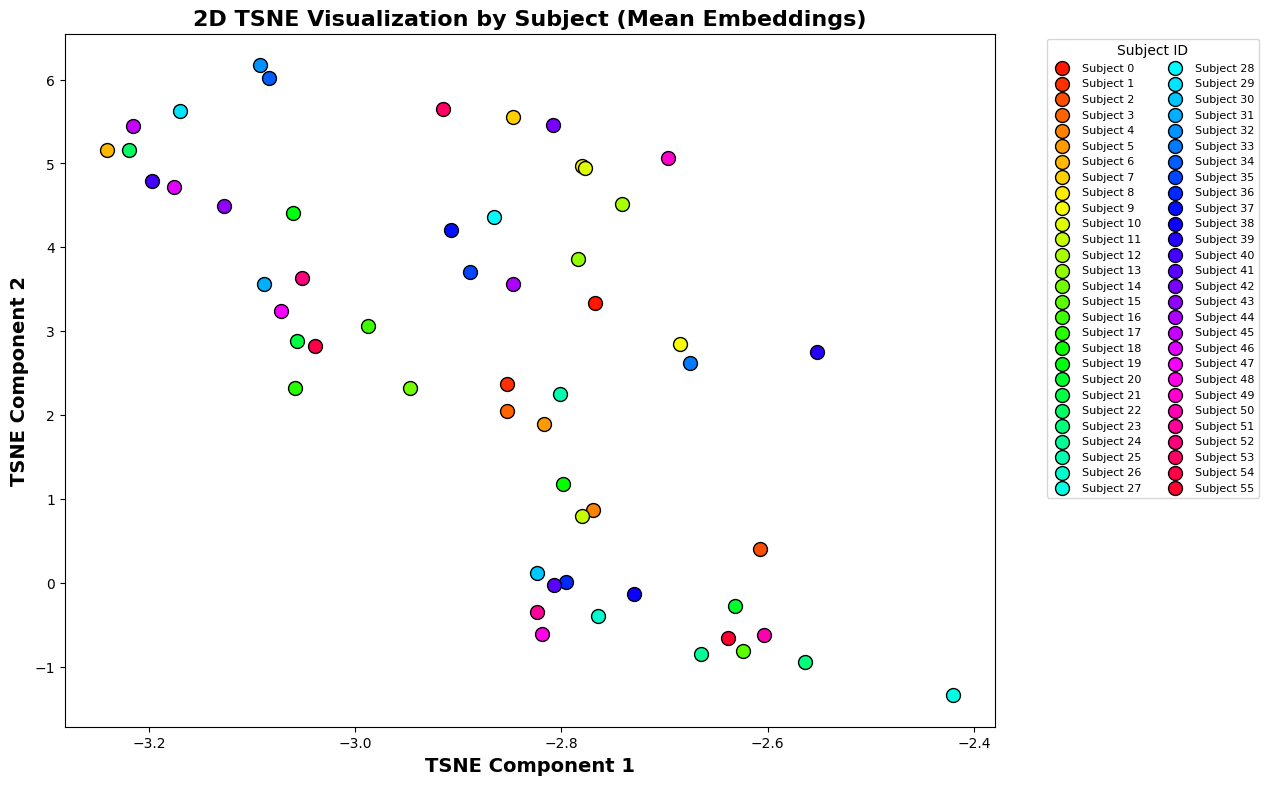
\includegraphics[width=0.48\textwidth, height=0.25\textheight]{Chapter2/Figures/ubfc_5bit__tsne.png}
        \label{fig:tsne_5bit_ubfc}
    }
    \hfill
    \subfigure[MSPM Dataset]{
        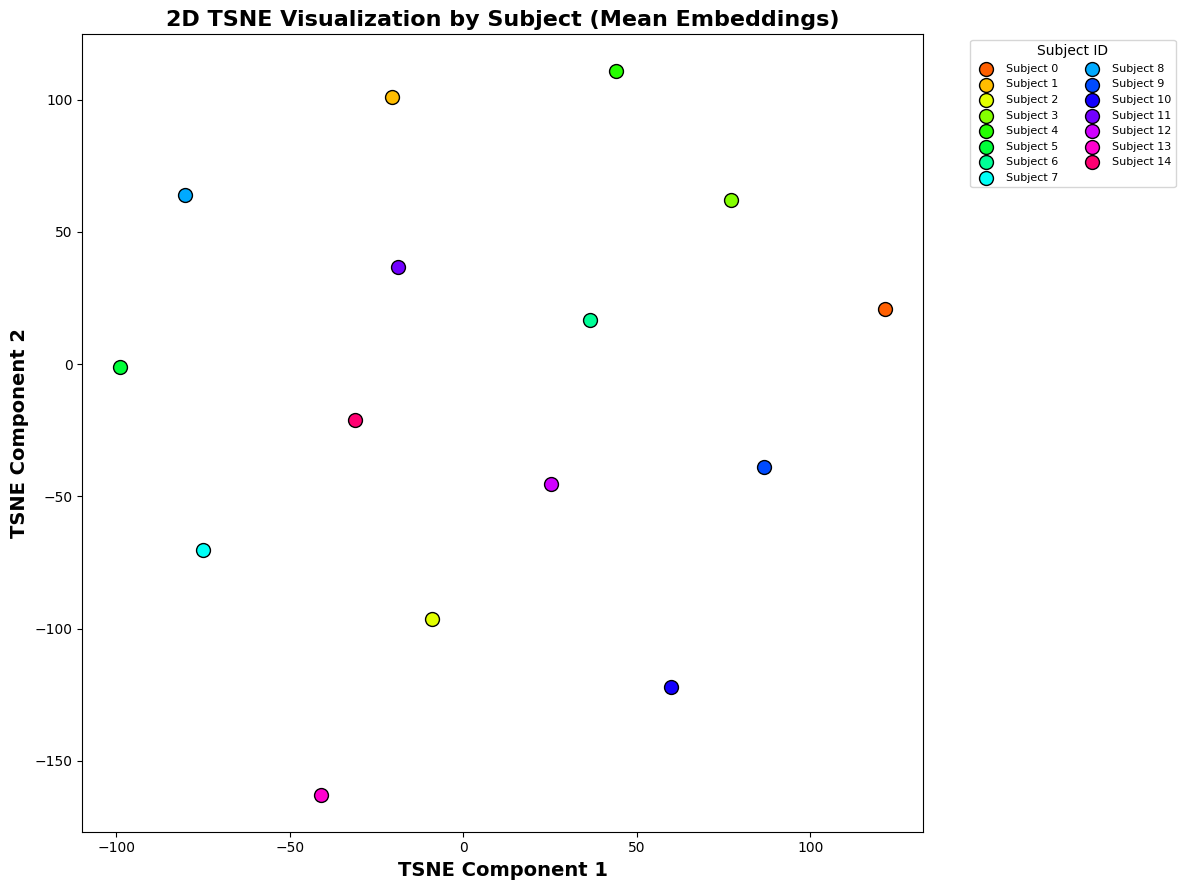
\includegraphics[width=0.48\textwidth, height=0.25\textheight]{Chapter2/Figures/mspm_5bit_tsne.png}
        \label{fig:tsne_5bit_mspm}
    }

    \caption{t-SNE visualizations of mean feature embeddings extracted from the UBFC and MSPM datasets after training with 5-bit quantization.}
    \label{fig:tsne_comparison_mean_embeddings}
\end{figure}




\subsection{Comparative Analysis}
\begin{table*}[h!]
\centering
\caption{EER and AUC for rPPG authentication on PURE, UBFC-Phys, and MSPM datasets under different signal lengths.}
\renewcommand{\arraystretch}{1.8}  % Increase row height for better readability
\resizebox{\textwidth}{!}{         % Scale only width, text stays proportional
\begin{tabular}{lcccccc}
\toprule
\multirow{2}{*}{\textbf{Signal Length}} & 
\multicolumn{2}{c}{\textbf{PURE}} & 
\multicolumn{2}{c}{\textbf{UBFC-Phys}} & 
\multicolumn{2}{c}{\textbf{MSPM}} \\
\cmidrule(lr){2-3} \cmidrule(lr){4-5} \cmidrule(lr){6-7}
& Intra-session & Cross-session & Intra-session & Cross-session & Intra-session & Cross-session \\
\midrule
20 heartbeats ($\sim$20 sec) & \textbf{0.07\%}/\textbf{95.54\%} & \textbf{0.18\%}/\textbf{84.74\%} & \textbf{0.48\%}/\textbf{50.62\%} & 0.50\%/50.42\% & \textbf{0.28\%}/\textbf{76.93\%} & \textbf{0.40\%}/\textbf{62.94\%} \\
10 heartbeats ($\sim$10 sec) & 0.11\%/92.12\% & 0.91\%/85.80\% & 0.49\%/49.87\% & 0.50\%/50.68\% & 0.48\%/51.72\% & 0.51\%/48.80\% \\
5 heartbeats ($\sim$5 sec) & 0.14\%/90.87\% & 0.21\%/84.79\% & 0.49\%/50.64\% & \textbf{0.49\%}/\textbf{50.64\%} & 0.50\%/50.00\% & 0.50\%/50.80\% \\
\bottomrule
\end{tabular}
}
\label{tab:eer_auc_rppg}
\end{table*}
For biometric identification, our CNN-based model demonstrates strong performance, particularly on the PURE dataset, where conditions are relatively controlled and stable. As shown in Table~\ref{tab:performance_pure_only}, the model achieves near-perfect identification metrics, confirming the discriminative power of the learned embeddings under 20 beats quantization scenarios. However, when evaluated on more challenging datasets such as UBFC-Phys, which include varying stress levels (low, mid, and high), the performance declines notably (Table~\ref{tab:eer_auc_rppg}). 

This performance drop is primarily attributed to physiological variability introduced under stress. The rPPG signals captured during these conditions tend to show greater temporal inconsistencies, reducing the repeatability and subject-specific uniqueness required for reliable biometric identification. In contrast to stable datasets like PURE, where the periodicity and amplitude patterns of rPPG signals remain consistent across sessions, the stress-induced changes in UBFC-Phys impact the embedding space and lead to overlapping or misclassified representations. This highlights a key limitation of current rPPG-based biometric systems: while effective under ideal conditions, their robustness under physiological or emotional variability remains an open challenge.

To support our findings, we further evaluated the model on the MSPM dataset, which includes recordings captured under varying real-world conditions. The model's reduced performance on this dataset reinforces the limitation of relying solely on rPPG signals for biometric identification in complex and uncontrolled environments.


In table\ref{tab:performance_pure_only}, we compare the rPPG biometrics with related biometric methods, when the signal length is 20 beats.
\begin{table}[htbp]
\centering
\caption{Performance comparison (EER and AUC) on the PURE dataset. The table compares biometric methods using face recognition (\ding{115}), cPPG biometrics (\ding{117}), and rPPG biometrics (\ding{72}). Lower EER and higher AUC indicate better performance.}
\resizebox{\textwidth}{!}{  
\begin{tabular}{lcc}
\toprule
\textbf{Biometric Methods} & \multicolumn{2}{c}{\textbf{EER↓ / AUC↑}} \\
\cmidrule(lr){2-3}
& \textbf{PURE (intra-sess)} & \textbf{PURE (cross-sess)} \\
\midrule
FaceNet~\cite{schroff2015facenet}  \ding{115}& 31.67\% / 66.67\% & 35.67\% / 65.11\% \\
Privacy-preserving FR~\cite{ji2022privacy} \ding{115} & 6.88\% / 91.27\% & 7.82\% / 90.77\% \\
Hwang2021~\cite{hwang2021variation} \ding{117} & \textbf{0\%} / \textbf{100\%} & {4.23\%} / \textbf{98.14\%} \\
Patil2018~\cite{patil2018non} \ding{72} & 4.00\% / 92.00\% & 32.68\% / 72.11\% \\
Sun2024~\cite{sun2024biometric}{ w/ rPPG training}\ding{72}& \textbf{0\%} / \textbf{100\%} & 11.68\% / 92.61\% \\
Sun2024~\cite{sun2024biometric}{ w/ rPPG-cPPG hybrid training}\ding{72} & \textbf{0\%} / \textbf{100\%} & 9.59\% / 93.70\% \\
\rowcolor{green!40}
\textbf{Ours }\ding{72} & {0.07\%} / {0.95\%} & \textbf{0.18\%} / 0.84\% \\
\bottomrule
\end{tabular}
}
\label{tab:performance_pure_only}
\end{table}




